\chapter{Introduction}
\label{ch:intro}
Digital imaging is omnipresent in today's world. There are many
handheld cameras available in the market that lets us take
high-definition pictures. Nevertheless, it is quite difficult to take
satisfying pictures from these cameras in certain scenarios, as we see
shortly.

\section{Motivation}

Consider a situation where we wish to inspect a dam by taking
pictures and following that up with offline post-processing.  We
would like to ensure that fissures, or cracks in the dam, along with
their respective positions, are flagged.  We cannot use a handheld
camera in this case as the approach to the dam is usually
inaccessible. As an additional example, next, consider
Figure~\ref{fig:orthographicView} which depicts a scene where
we wish to capture images of a large wall. The perspective view of the
wall doesn't provide details of objects such as the indicated dial.

In both of these cases, we wish to image the wall orthographically, i.e.,
by keeping the viewing direction normal to the wall.  Further, the
camera must be close to the wall if we are to capture details; as a
corollary, this implies that we have to move the camera along the two
dimensions of the wall to image the entire surface.

\begin{figure}[h!]
\centering
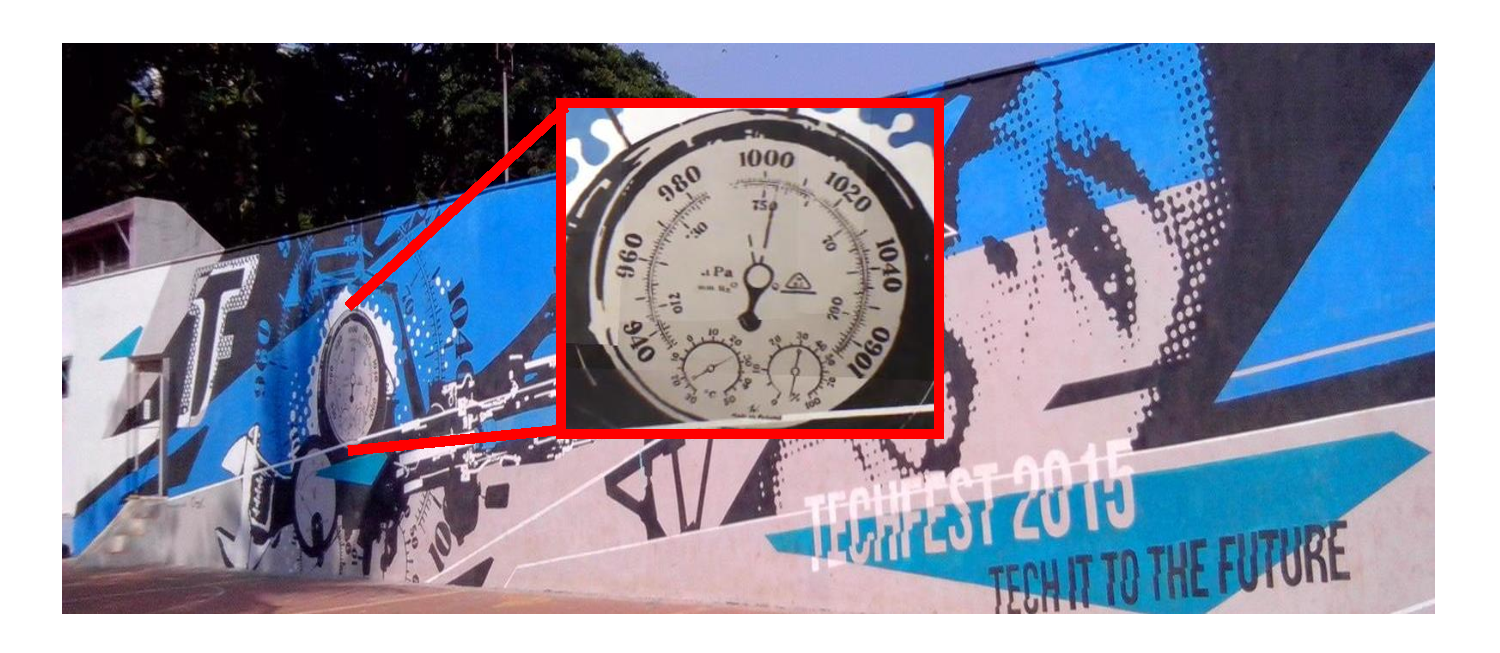
\includegraphics[width=0.98\linewidth]{figures/orthographicView}
\caption[Problems in imaging a large scene using a handheld
  camera]{Illustration of problems in imaging large planar scene with
  a handheld camera. A 40 feet wall captured with a handheld camera
  from a distance doesn't reveal details of the dial shown in the
  box. We wish to image such large planar structures by placing the
  camera close to and normal to the plane and later mosaic individual
  pieces.}
\label{fig:orthographicView}
\end{figure}

\emph{Quadcopters} (quadrotor helicopters) can be used to image large
planar surfaces from a close distance such as dams. Note that, as
mentioned above, we cannot capture an orthographic view of the entire
large planar surface from such distance in a single frame. In fact, we
will get a battery of images to encompass the whole scene
orthographically. These images must be stitched to get a panoramic
view.  Such a view will allow us to do post-processing as desired.

Panoramic construction requires alignment of overlapped
images~\cite{Brown03}.  These methods rely significantly on finding
common \textit{features} in overlapped images so as to establish
appropriate warps to register or align the images together. When we
attempt to use these methods for the purposes mentioned here, we noted
that there are cases where the imaged surface contains large textureless
regions. We term these regions as \emph{vacant spaces}. For example, in an art
gallery example shown in Figure~\ref{fig:indoor}, we have exhibits separated by
``empty spaces''. Notice that in Figure~\ref{fig:indoor}, images $\alpha$,
$\alpha'$, $\beta$, and $\beta'$ have `features', while images A, B, and C do
not have any significant features.  We can align images $\alpha$ with $\alpha
'$ as well as $\beta$ with $\beta '$, but not $\alpha$ with A, or C with
$\beta$.  Similarly, we cannot align A with B or B with C. Large homogeneous
vacant spaces result in scene regions that have little or no matches between
many significant images. As a result, we cannot create a panorama using
traditional mosaicing methods. In our example, we cannot build a bridge between
$\alpha$ and $\beta$ due to the presence of vacant space, which results in
disconnected components. Hence, there is a requirement of a method that can
infer positions to assist in mosaicing.  In this thesis, we propose the use of
quadcopters.

\begin{figure}[h!]
\centering
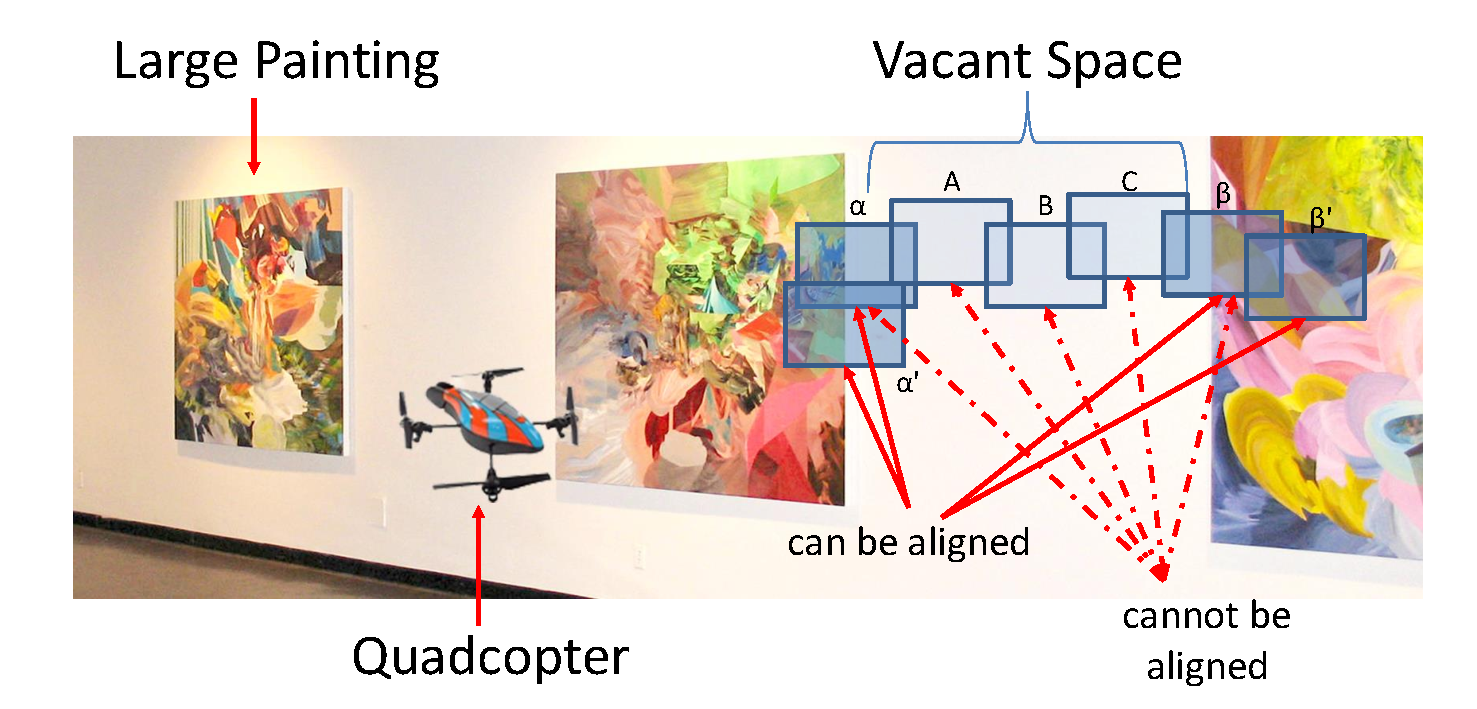
\includegraphics[width=0.98\linewidth]{figures/vacantSpaces/indoor}
\caption[Vacant spaces problem in art gallery]{Vacant spaces are
  encountered in the imaging of this scene. When individual portions
  are captured by a quadcopter, how does one create the complete
  mosaic, given that common features are unavailable? In this example,
  $\alpha$ and $\alpha '$ can be aligned, and so can $\beta$ and
  $\beta '$. This is not true for the constituents of the 5-tuple ($\alpha$, A,
  B, C, and $\beta$).}
\label{fig:indoor}
\end{figure}
    
Now, consider yet another situation where, with quadcopters as the
instrument, we would like to capture the paintings or murals on large
walls of a temple. We would like to ensure that details of the
painting are captured in a sufficient high definition. Often, temple
paintings are arranged in sequential order, depicting a particular
mythological story. In such cases, we would like to capture these
paintings spread over multiple walls and create an \emph{unrolled}
view of the scene where we get the output mosaic of the input scene as if it is
present on a single plane.  We have to make sure that capturing is done in a
manner such that full scene is imaged in minimum time to reduce inconvenience.

In such cases, we have to navigate the quadcopter smoothly to image
large multiplanar surfaces from a close distance. We examine current
options available for the navigation and control of quadcopter.  Most
predominantly, First Person View (FPV) controllers are available with
current quadcopters. However, considerable manual adjustments are
needed using the FPV to ensure specific depth, impacting the time of
capture. Next, if we have to capture large surfaces, the manual effort
is non-trivial.  Finally, as always with a manual procedure (and from
our experience), there is a high probability of collision during
these adjustments which may cause damage to the precious monuments.

The need for more control has led to software applications, typically
mobile based, for semi-autonomous navigation of a quadcopter.  As an
example, we can use these mobile applications to do basic maneuvers
(e.g., ``go from position X to position Y''). While these applications
are satisfactory for casual situations such as taking selfies, they
are unsuitable for the problem at hand.  For example, we cannot ensure
an orthographic view from a specific depth, even while traveling
autonomously along two dimensions of a large planar structure.  These
applications are not sufficiently autonomous either, to navigate the
quadcopter autonomously. Hence, there is a requirement of developing a
stable technique for autonomous navigation and control of quadcopters
in indoor as well as outdoor scenarios.
 
Imaging large multiplanar surfaces using a single quadcopter in one
flight is not always feasible due to battery constraints. In such
cases, one may use multiple quadcopters in collaboration. The
identification of every quadcopter under motion is essential for using
multiple quadcopters. Fiducial markers such as ARTag have been used to
identify objects. However, due to the swift motion of a quadcopter, a
significant amount of motion blur is introduced. If such fiducials are
placed on non-stationery objects, they do not get recognized because
recognition of these fiducials depends on the detection of geometric
patterns such as lines, corners, etc.  Hence, there is a necessity of
developing blur resilient fiducials which can be recognized robustly
when placed on swift moving objects such as quadcopters.

\section*{Problem Statement}
\textit{The problem of autonomous navigation of quadcopters to image
  multiplanar surfaces containing vacant spaces with correct
  identification of individual quadcopter forms the problem statement
  of the work presented in this thesis.}

We decompose our problem of mosaicing a multiplanar scene containing
vacant spaces through the autonomous navigation of one or more
quadcopters into the following steps:
\begin{enumerate}
  \item Mosaicing a \textit{single} planar scene, possibly containing vacant
  spaces.
  \item Autonomous navigation of quadcopter for imaging a multiplanar scene.
	\begin{enumerate}
  		\item Path planning for imaging each planar region in a multiplanar scene.
	\end{enumerate}
  \item Unrolling scenes spread over multiple planes.
  \item Devising a mechanism for robust recognition of quadcopters under swift
  motion.
\end{enumerate}
Each of these steps is non-trivial and challenging as explained in
next section. In this thesis, we deal with these steps by leveraging
the additional information available onboard the quadcopter.

In considering quadcopters, we briefly consider factors for the selection of
the imaging instrument. We require at a minimum three characteristics in
quadcopters to achieve the goal of autonomous navigation. First, quadcopters
should have a camera with reasonable resolution (at least 1080 x 720
pixels). Second, they should be able to communicate with a computer
through a well-established protocol. Third, we should be able to fly
them indoors as well as outdoors. The cost is clearly a factor once
these three requirements are satisfied.

The first requirement is met in most of the quadcopters, but only a
few quadcopters satisfy the second and third requirements
simultaneously. For example, the DJI Phantom 4, costing around 1200
USD has a camera mounted on 3-axis gimbal coupled with a gyroscope. It
enables us to take very stable videos while flying. There are FPV
controllers as well as mobile applications available for
semi-autonomous navigation of DJI Phantom 4. But as discussed earlier,
these options are not useful in solving our problem.  Also, there is
inadequate open-source software support for autonomous navigation of
DJI Phantom 4.

Some quadcopters have a GPS to assist navigation. But we cannot use
GPS facility in an indoor scenario. Even if the GPS signal is
available, we cannot rely only on GPS for navigation of quadcopters in
outdoor scenarios due to GPS jamming and the spurious GPS signals.

Octocopters such as DJI S1000 have excellent flight control as well as
stability. But due to their bulky nature (weight around 11Kg), we
cannot use it in indoor areas. There are a few non-commercial
quadcopter systems which have gained focus, e.g., the team at the
University of Pennsylvania has developed a series of quadcopters
capable of doing unbelievable maneuvers. However, such systems use
high-speed motion camera systems such as Vicon to find out the pose of
the quadcopter in motion. Hence, we cannot use them in uncontrolled
environments.

Parrot's ARDrone and Bebop are two reasonably priced (USD 350 and USD
700 respectively) quadcopters having HD camera with resolution 1280 x 720
pixels. Though they are lightweight (0.42 kg) compared to the DJI Phantom 4
(around 1.4kg), they are robust enough to withstand outdoor conditions. ARDrone
streams a WiFi hotspot to which any computer can be connected. Parrot has also
released an SDK which is essential to do interfacing with these quadcopters.
When I had started work on quadcopters (in mid-2013), Parrot's Bebop was not
available. Hence, I have used Parrot's ARDrone 2.0 for my research work
presented in this thesis.

\section*{Challenges}
\label{sec:challenges}
The challenges which make our problem interesting to solve are as follows.

\begin{itemize}
  
\begin{figure}[h!]
\centering
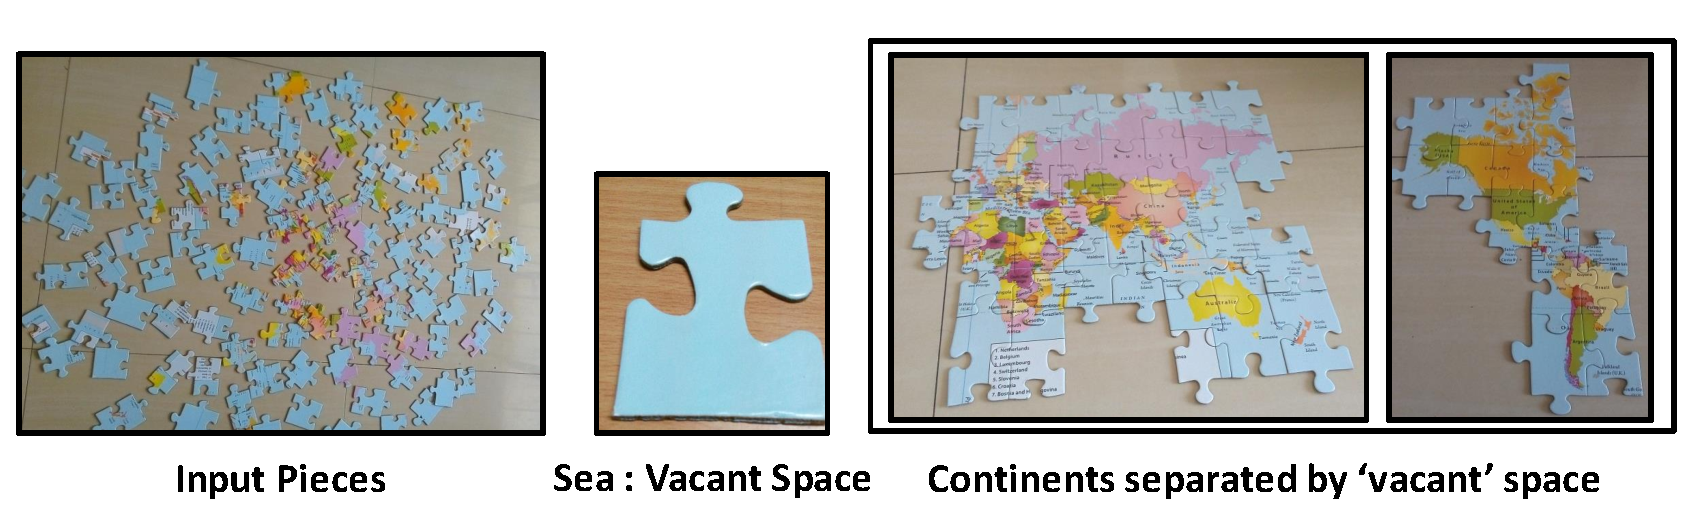
\includegraphics[width=0.98\linewidth]{figures/vacantSpaces}
\caption[Jigsaw Puzzle as a mosaicing problem]{Jigsaw Puzzle as a mosaicing
problem. Individual pieces (Left) of a jigsaw puzzle can be thought of
constituent images of mosaic. Due to featureless regions corresponding to seas,
(shown in Middle), it is problematic to join ``Americas'' (Right) with the
remaining continents. We have to use our knowledge about geography to complete
the puzzle. Purely from a matching perspective, Americas could well come to the
left or right in this puzzle.}
\label{fig:vacantSpaces}
\end{figure}
  
  \item \textbf{Vacant spaces and regions with confusing features:}
    Mosaicing a scene is similar to solving a jigsaw puzzle like the one shown in
  Figure~\ref{fig:vacantSpaces}. Here, individual pieces of the puzzle can be
  thought of as constituent images in a mosaic. We have to match
  pieces and join them. This is similar to the stitching algorithms
  which find matches in two images for estimating the relative position of one
  image with respect to another image. Normally, pieces can be placed at their
  correct positions by matching a color, texture, as wells as a shape on the piece,
  e.g., if there is a red colored piece, we can consider only other red
  colored pieces whose boundaries match with the first piece. The blank
  pieces representing the seas make such puzzles hard to solve. While solving
  jigsaw puzzle containing blank pieces, we could build the parts of the
  puzzle, e.g., ``Americas" and rest of the world as shown in
  Figure~\ref{fig:vacantSpaces}. However, we cannot place these parts at
  their respective positions as we cannot match these parts with blank
  pieces to complete the puzzle. Here, we have to use additional positional
  information (e.g., geography in the puzzle shown in
  Figure~\ref{fig:vacantSpaces}) to join different parts separated by
  vacant spaces. In general, images containing very less or no features are
  difficult to match.

  The standard mosaicing method uses feature matching algorithms for
  estimating the homography between two images. Feature matching algorithms
  require detection of sufficient features in both images. However, scenes like
  Figure~\ref{fig:vacantSpacesExample}(left) contain large regions with vacant
  spaces. Such regions result in very few (or almost zero) features which pose
  a problem for stitching images containing such regions. The output (shown in
  Figure~\ref{fig:vacantSpacesExample}-right) of Adobe Photoshop~\cite{photoshop}, 
  a popular mosaicing software showcases the inability to handle vacant spaces.
  
 \begin{figure}[h!]
\centering
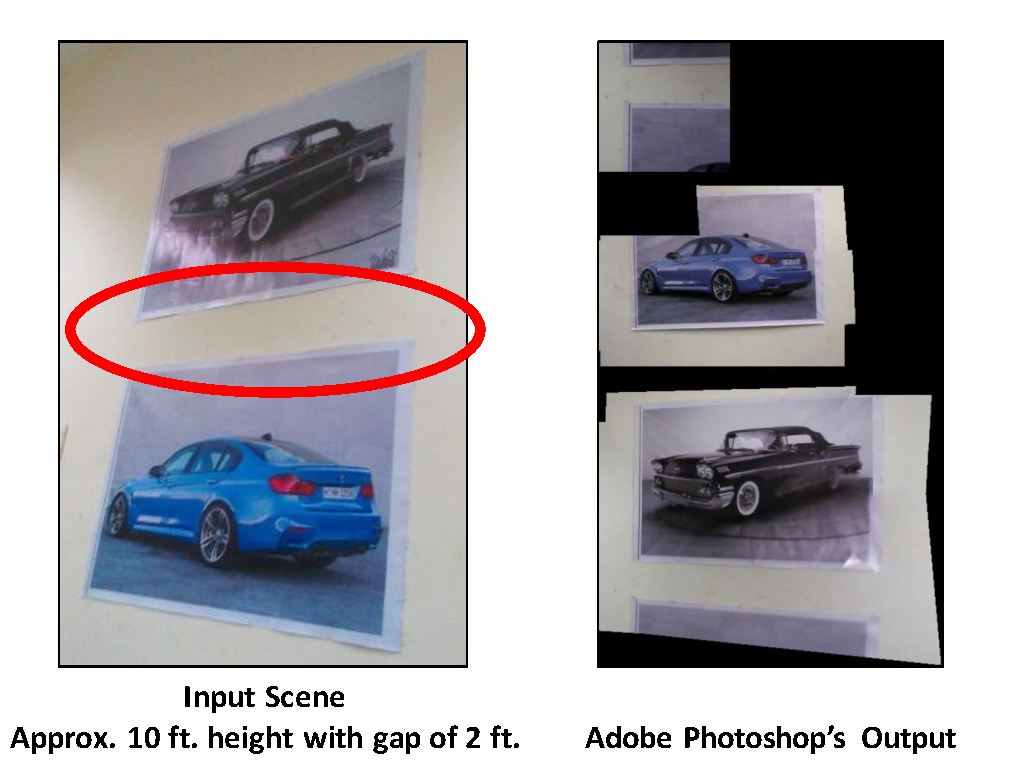
\includegraphics[width=0.98\linewidth]{figures/vacantSpacesExample}
 \caption[Problem of mosaicing scene with vacant spaces using Adobe
 Photoshop]{Is Mosaicing problem solved? Standard stitchers such as Adobe
 Photoshop~\cite{photoshop} cannot stitch images which have none or very little
 features in common. Left: there is an input scene containing vacant space
 separating the two posters (indicated by the red oval). Right: Adobe Photoshop
 outputs individual pieces instead of complete mosaic as feature matching
 algorithm fails.}
\label{fig:vacantSpacesExample}
\end{figure}
 
  There is another problem with standard stitching algorithms due to 
  reliance on feature matching. The feature matching algorithm gets confused
  when parts of the scene are repeated. It results in images which are not
  taken from adjacent positions being stitched together.
  Figure~\ref{fig:confusingFeatures} shows output of
  AutoStitch~\cite{autostitch}, the state of the art stitcher, on an input scene
  containing repetitive patterns. It can be seen that images taken from
  positions far apart from each other get stitched together as the matching
  algorithm matches features from those images.

\begin{figure}[h!]
\centering
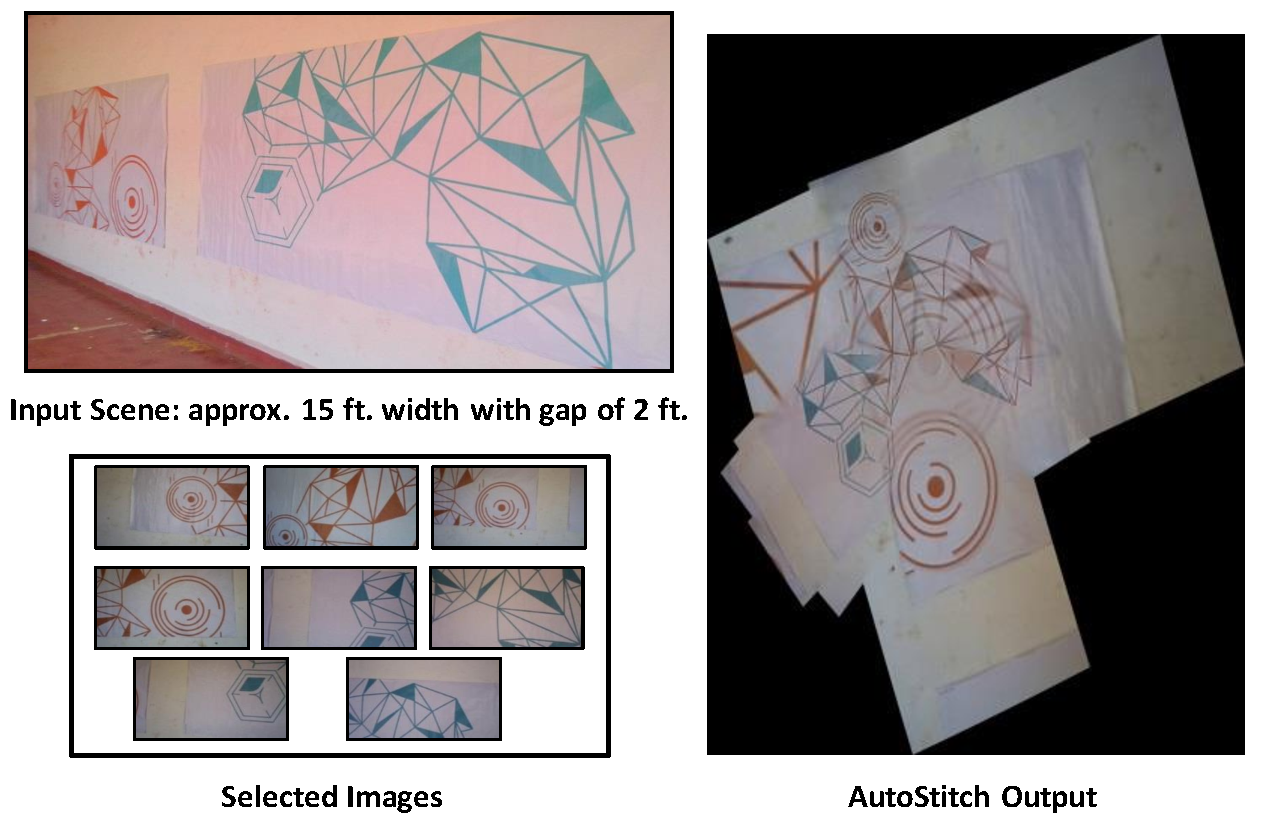
\includegraphics[width=0.98\linewidth]{figures/confusingFeaturesExample}
\caption[Problem of confusing features in AutoStitch]{Repetitive patterns in the
input scene pose a challenge for standard mosaicing methods such as
AutoStitch~\cite{autostitch}. Images taken from positions far apart from each
other get stitched together as matching algorithm matches features from those
images.}
\label{fig:confusingFeatures}
\end{figure}  

  \item \textbf{Control and navigation of an inexpensive quadcopter:}
  Inexpensive quadcopters like Parrot's ARDrone are agile and can do
  several maneuvers swiftly. However, manually controlling a quadcopter to image large
  planar regions smoothly by keeping a constant distance from the imaging plane
  is very difficult because of the tendency of quadcopter to drift from its
  desired position. Hence, there is a requirement of a mechanism for autonomous navigation of
  quadcopter. One does not have to image the scene continuously while navigating
  the quadcopter as too many pictures are redundant. We have to estimate the
  optimal number of positions of the quadcopter from where it can take images,
  even while ensuring that captured images encompass the scene.
  
  \item \textbf{Building a scale accurate 3D map of the environment in
  real-time:} A quadcopter has to be maneuvered along an estimated path such
  that it will cover the input scene in minimum time. We require accurate
  3D coordinates of the region to be imaged on the fly for doing efficient path
  planning. Researchers generally use RGBD cameras such as the Microsoft
  Kinect~\cite{Zhang:2012} for getting a 3D map of the environment. However,
  due to payload restrictions as well as battery requirements, it is not
  efficient to put such cameras on top of a quadcopter like ARDrone. Structure
  from Motion (SfM) techniques can build such a 3D map, but due to the
  real-time requirement, we cannot use such techniques. There are various
  methods based on popular techniques such as Simultaneous Localization and
  Mapping (SLAM) or Parallel Tracking and Mapping (PTAM) for creating a 3D map
  of the environment. However, most of these methods, e.g.,~\cite{klein}, lack
  the accuracy in scale estimation due to complete reliance on visual feedback,
  resulting in an erroneous 3D map. Engel et al.~\cite{engel} have developed a
  method which fuses IMU measurements with the PTAM measurements, to create a
  3D map for camera-based navigation of a quadcopter. However, it is not
  sufficiently precise for our purposes due to inaccuracies in scale.
  
  \item \textbf{Robust detection of multiplanar bounded regions in real-time:} 
  Multiplanar imaging through quadcopter requires detection of multiplanar
  bounded regions in real-time. There are a few methods like
  multiRANSAC~\cite{zuliani}, J-linkage~\cite{jlinkage},
  T-linkage~\cite{tlinkage} in the literature for detection of multiple planes
  from the input data. These methods do not output the boundaries of planar
  regions. They only output the estimated planes from the input 3D points using
  geometric affinity of points towards individual planes. Also, these methods
  have not considered the validity of boundaries of planar regions to remove
  noisy points. As a result, such noisy points get clustered into wrong planes,
  extending boundaries of planar regions incorrectly.
  Figure~\ref{fig:jlinkageProblem} illustrates this problem. Points marked by
  black oval are the result of erroneous estimations by PTAM, i.e., marked
  points labeled as plane B actually belong to the plane A and vice-versa. 
  Since their geometric affinity is towards opposite planes, they are labeled
  incorrectly.

\begin{figure}[h!]
\centering
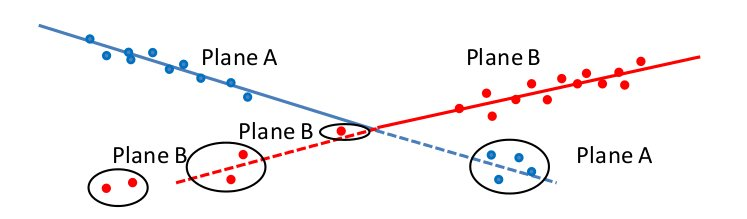
\includegraphics[width=0.98\linewidth]{figures/multiplanar/JlinkageProblem}
\caption{Problem in J-linkage clustering. J-linkage doesn't use validity of plane
boundaries to cluster points to correct planes. Points marked by black ovals
are the result of erroneous estimations by PTAM. Since their geometric
affinity is towards opposite planes, they are labeled incorrectly.}
\label{fig:jlinkageProblem}
\end{figure}

  \item \textbf{Identification of a quadcopter under motion:}
  Imaging large multiplanar scenes using a single quadcopter is difficult 
  due to the insufficient power available in the battery. Multiple 
  quadcopters can be used in such scenarios to work in collaboration. Each
  quadcopter requires to be distinguished. The movement of quadcopter like
  ARDrone is quite jerky which results in motion blur in images of quadcopters.
  It makes tracking of such quadcopters challenging. Normally, we can place
  fiducials on the quadcopter to keep track. ARTag~\cite{Fiala05} is preferred
  over other fiducials like ARToolkit~\cite{ARToolkit02}, PiTag~\cite{Pitag13},
  etc. as the recognition rate of ARTag is better than other existing fiducials.
  However, none of these fiducials are recognized in the presence of motion
  blur. Figure \ref{fig:ARTagBlur} demonstrates the problem in recognition of
  ARTag under motion blur. Figure \ref{fig:ARTagBlur} (Left) shows that ARTags
  get recognized (indicated by green rectangles) in the absence of blur in
  captured images. However, when there is a significant amount of blur, ARTags cannot be
  recognized (Figure \ref{fig:ARTagBlur} (Right)).
  
\begin{figure}[h!]
\centering
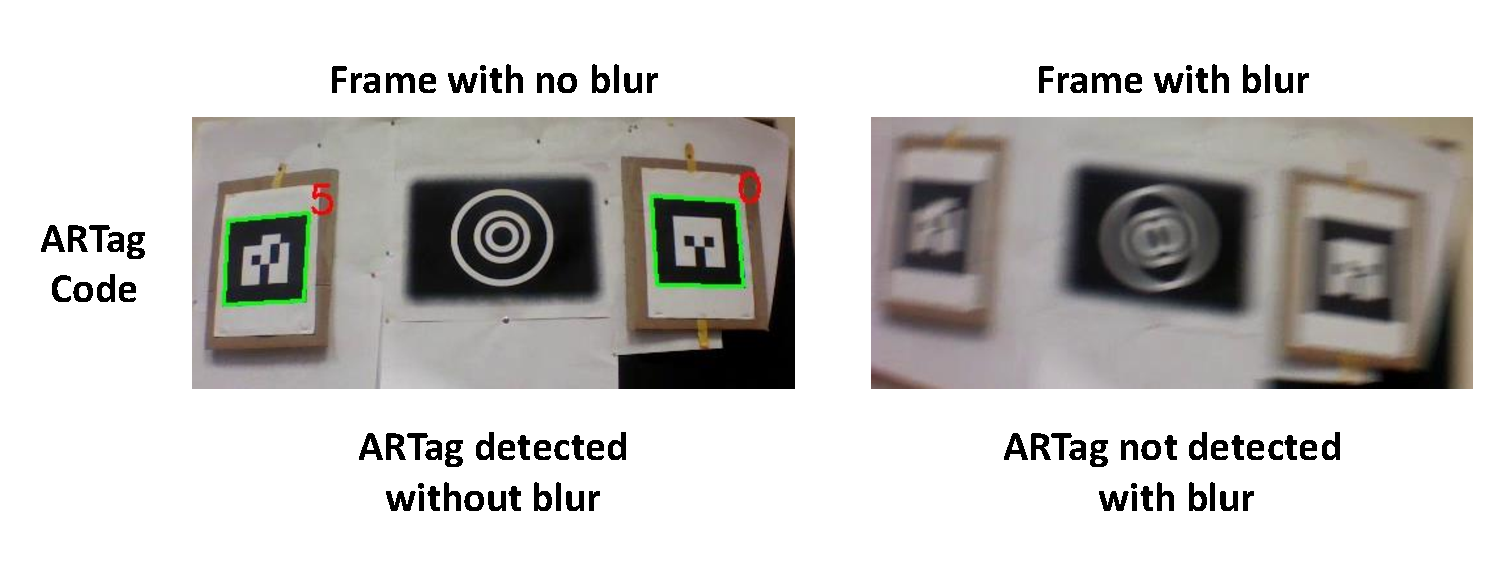
\includegraphics[width=0.98\linewidth]{figures/fiducial/ARTagBlur}
\caption[Problem of motion blur in ARTag]{Illustration of problem with ARTag.
There are two ARTags in the scene.
When there is no blur in the captured image (Left), both ARTags are recognized
(indicated by green rectangle). When there is motion blur in the captured
image (Right), neither of the two tags are recognized.}
\label{fig:ARTagBlur}
\end{figure}

\end{itemize}

\section{Contributions of this thesis}
\begin{figure}[h!]
\centering
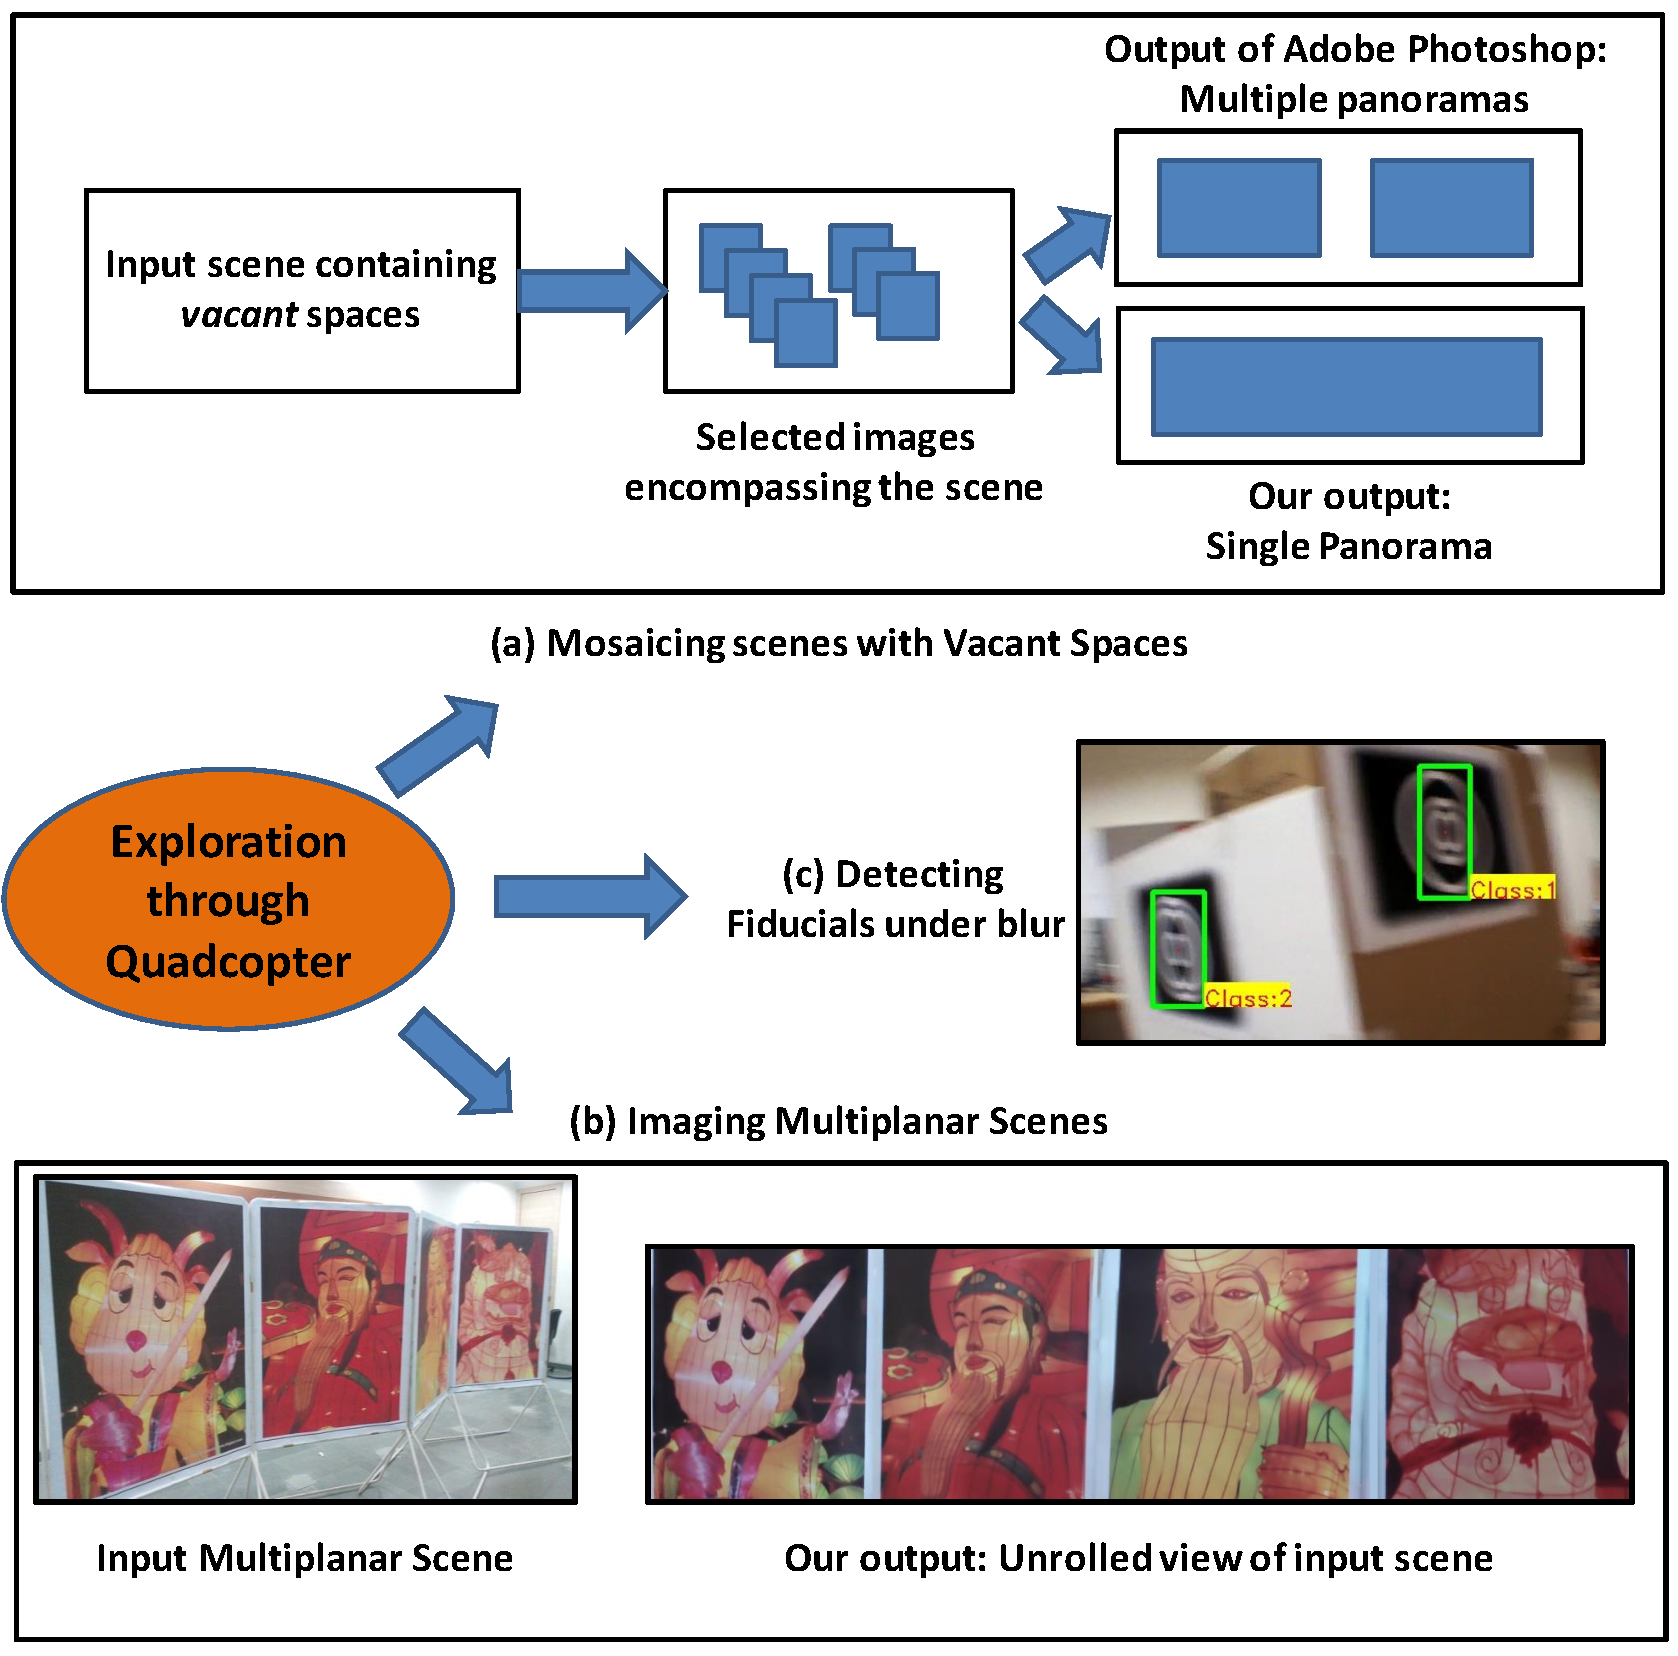
\includegraphics[width=0.98\linewidth]{figures/contributions2}
\caption[Contributions]{Our work involves techniques required for imaging
multiplanar surfaces through one or more quadcopters. (a) Mosaicing of a scene containing
vacant spaces. Two exhibits on a wall are separated by  a large vacant space
which makes homography based stitching methods ineffective. (b) Imaging
of a multiplanar scene through quadcopter. We imaged a multiplanar scene in such
a way that content on each plane is imaged with an orthographic view. Later we
combined a mosaic from each planar bounded region to get the  unrolled view of
an overall scene. (c) Blur-resilient fiducials being detected in the
presence of motion blur, even from oblique angles.}
\label{fig:contributions}
\end{figure}

As shown in Figure \ref{fig:contributions}, we have developed an integrated solution to
explore scenes spread over single or multiplanar scenes through quadcopter. To
the best of our knowledge, we are the first 
\begin{itemize}
  \item To mosaic scenes with vacant spaces using a quadcopter  
  \item To image scenes spread over multiple planes autonomously using a quadcopter  
\end{itemize}

Specific contributions made to achieve this goal and to address the above
mentioned challenges are:\\

\subsection{Mosaicing Scenes with Vacant Spaces}
\begin{figure}[h!]
	\centering
	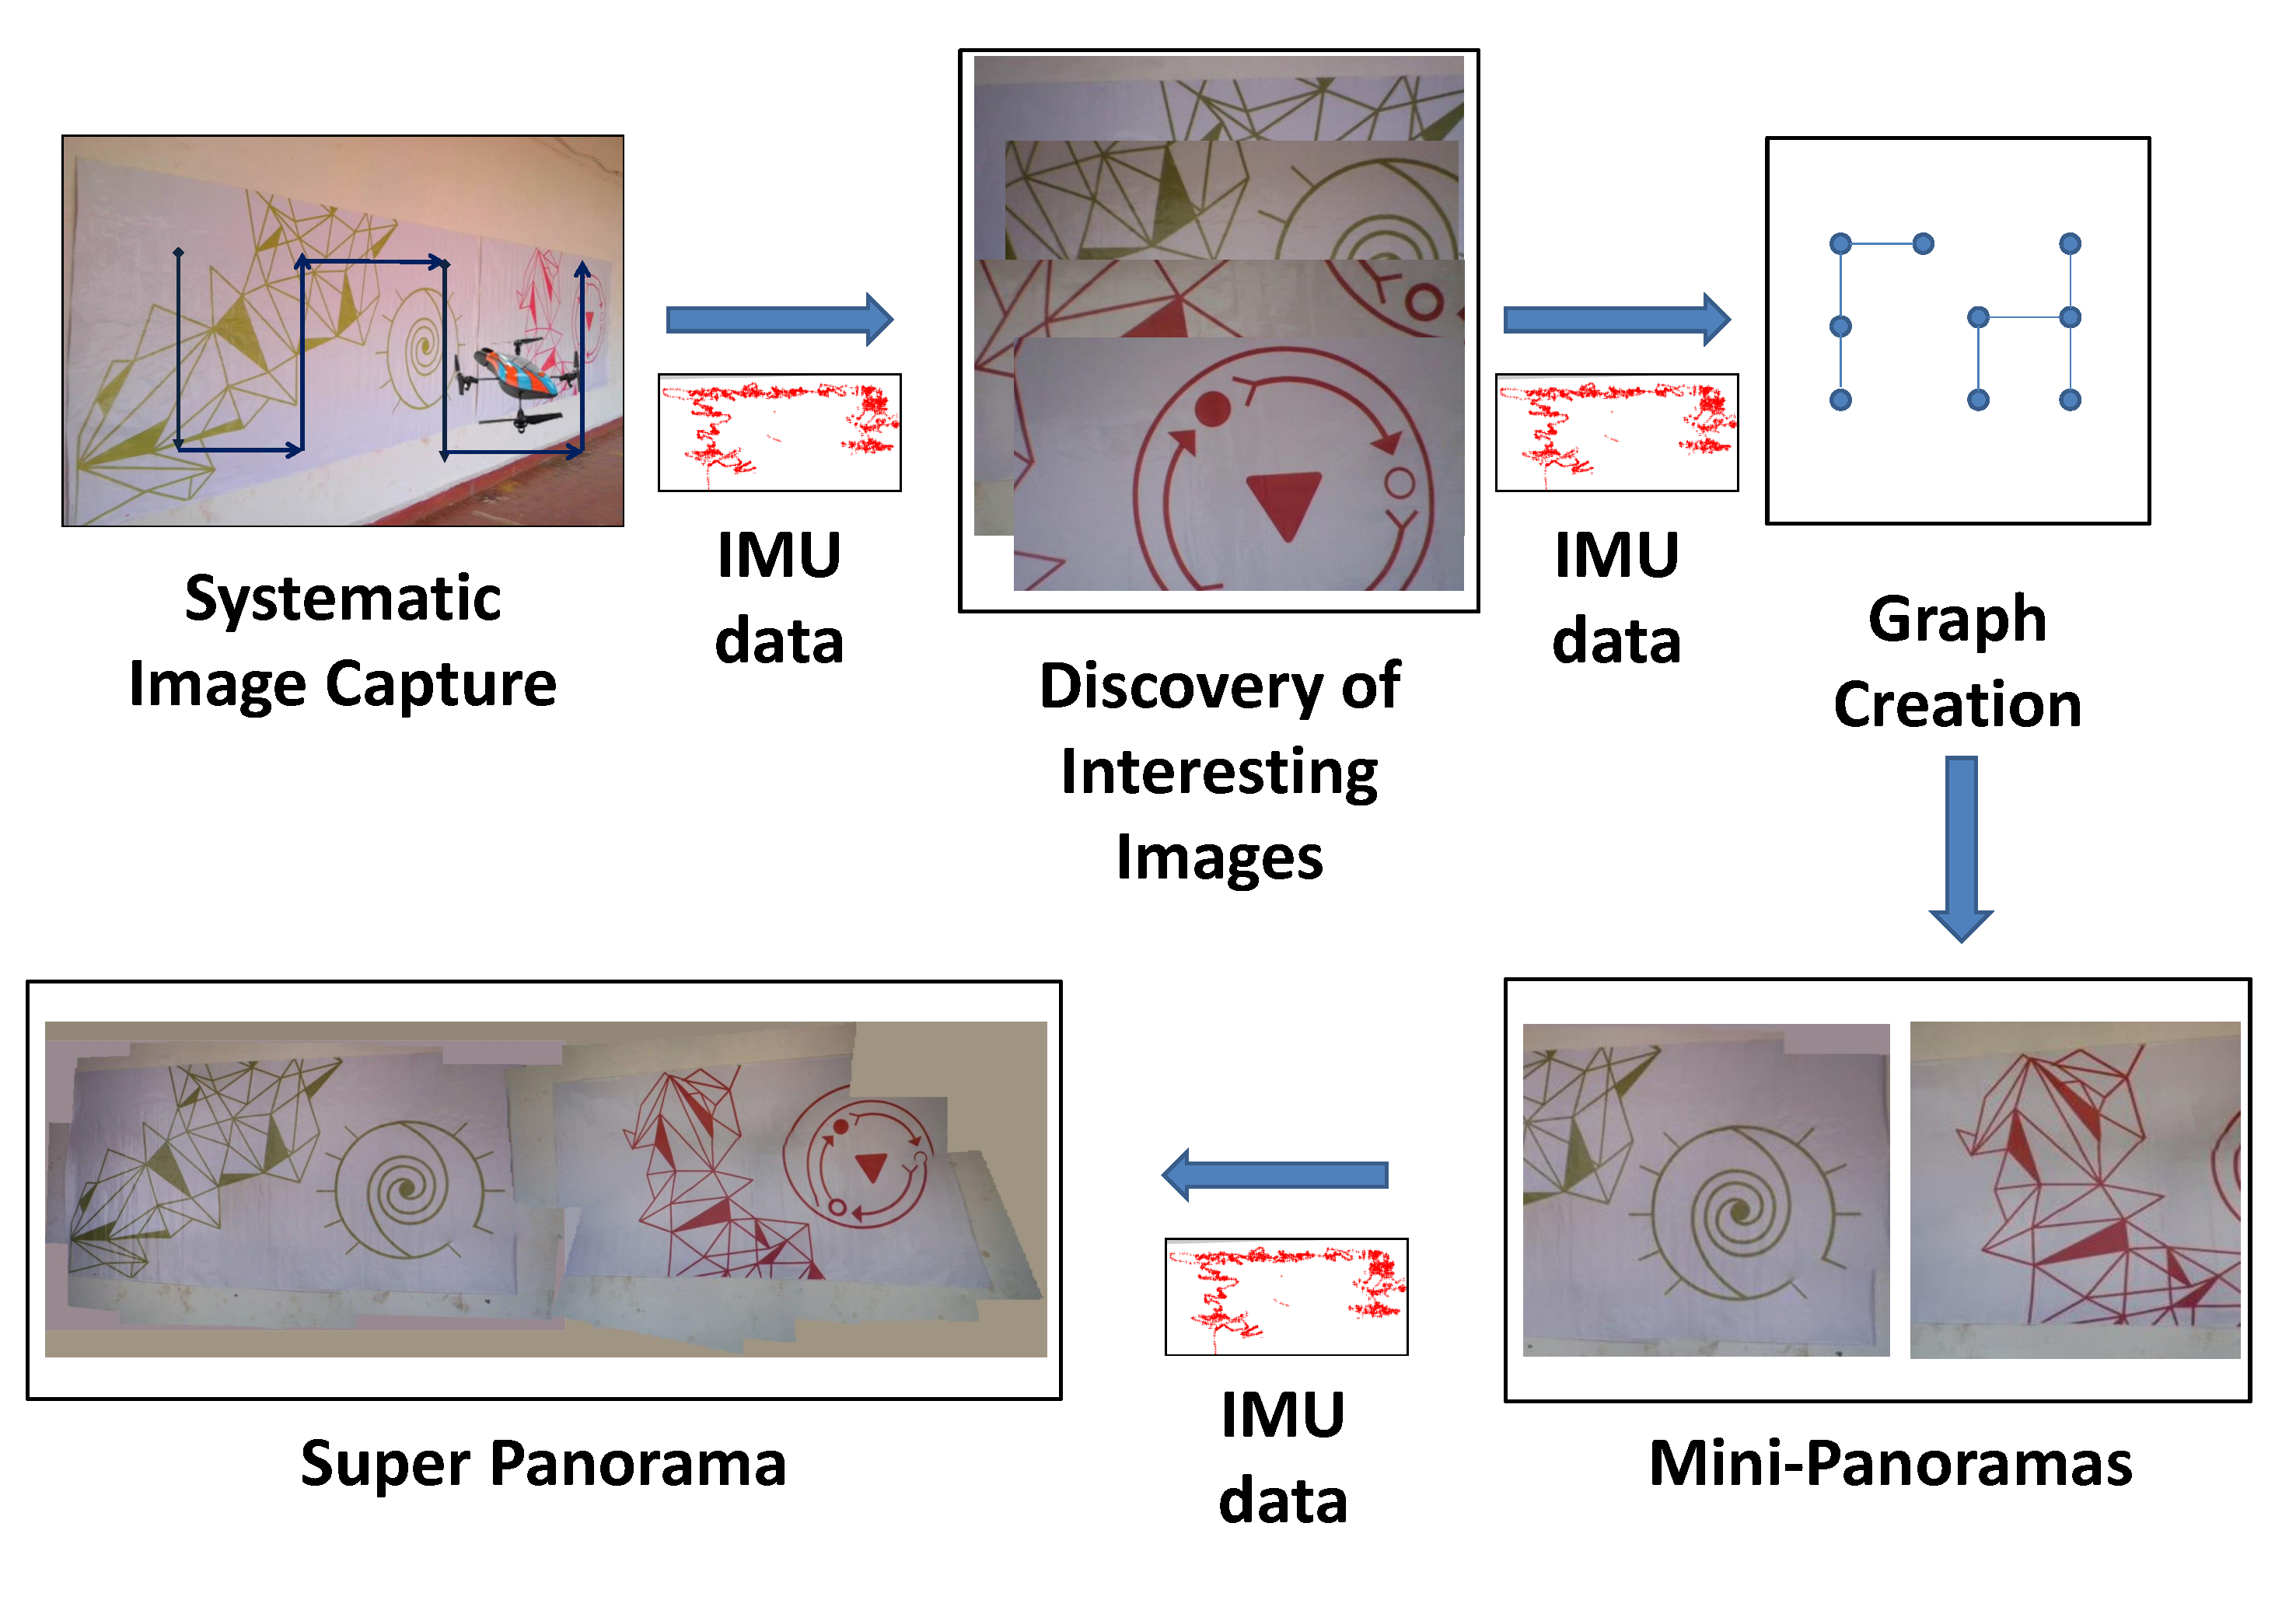
\includegraphics[width=0.98\linewidth]{figures/vacantSpaces/Workflow}
	\caption[Workflow]{ Overview of mosaicing scenes with vacant spaces: Input
	imagery is systematically acquired (top left) by a quadcopter.  In the next
    step, interesting images are found by clustering the video into
    regions based on positional data.  A graph is constructed using
    proximal images. For each connected component in a graph, standard
    stitching techniques are used to create mini-panoramas which are
    then joined together into a super panorama 
    again using IMU data.}
    \label{fig:vaccantSpaces_workflow} 
  \end{figure}
  
  We propose to solve the vacant space problem by using additional information
  available from an inexpensive quadcopter.  Quadcopters contain an inertial
measurement unit (IMU) that has positional information. We use the positional
information from IMU primarily for two purposes:
\begin{enumerate}
\item \textbf{Selection and ordering of images:}
We use the IMU data to select representative images from the video and arrange
them into rectangular grid according to the `spatial' neighborhood. It also
  disambiguates situations when multiple images that are spatially distant,
  have similar, repeated features.

\item \textbf{Super-panorama:} Whenever there are no features in
  the overlap region of two images, we use the IMU data to find the
  relative position of one mini-panorama with respect to another.
\end{enumerate}

However, IMU data on a quadcopter cannot be relied exclusively, or sometimes at
all, especially on inexpensive devices. Our experiments indicate that roll
and pitch angles (depending on the distances involved) may be completely off,
and so can the physical coordinates.  This is a consequence of jerky,
swift movements.  Complementing the IMU with information gleaned from
vision algorithms, however, may be a useful practice.

The method adopted is pictorially depicted in the overview shown in
Figure~\ref{fig:vaccantSpaces_workflow}.  In brief, we systematically acquire a
video of the scene, reduce the input video to a manageable number of images,
and finally, combine the images acquired from different positions into a mosaic. 

The result on a sample scene is shown in Figure~\ref{fig:vacantSpaces_result}.
In this experiment, the input stream had about 9000 input images.  Our selection algorithm
 pruned the video into $N=13$ images. A sample of the selected images are seen
 in Figure~\ref{fig:vacantSpaces_result}(a).  The scene as captured by a
 smartphone can also be seen, as well as the outputs of the state of the art
 stitchers, viz., AutoStitch~\cite{autostitch} and Adobe
 PhotoShop~\cite{photoshop}. Note that AutoStitch~\cite{autostitch} is only able
 to stitch the upper half of the scene.  Our result
 Figure~\ref{fig:vacantSpaces_result}(e) clearly stands out in comparison.\\
  
  \begin{figure}[h!]
	\centering
	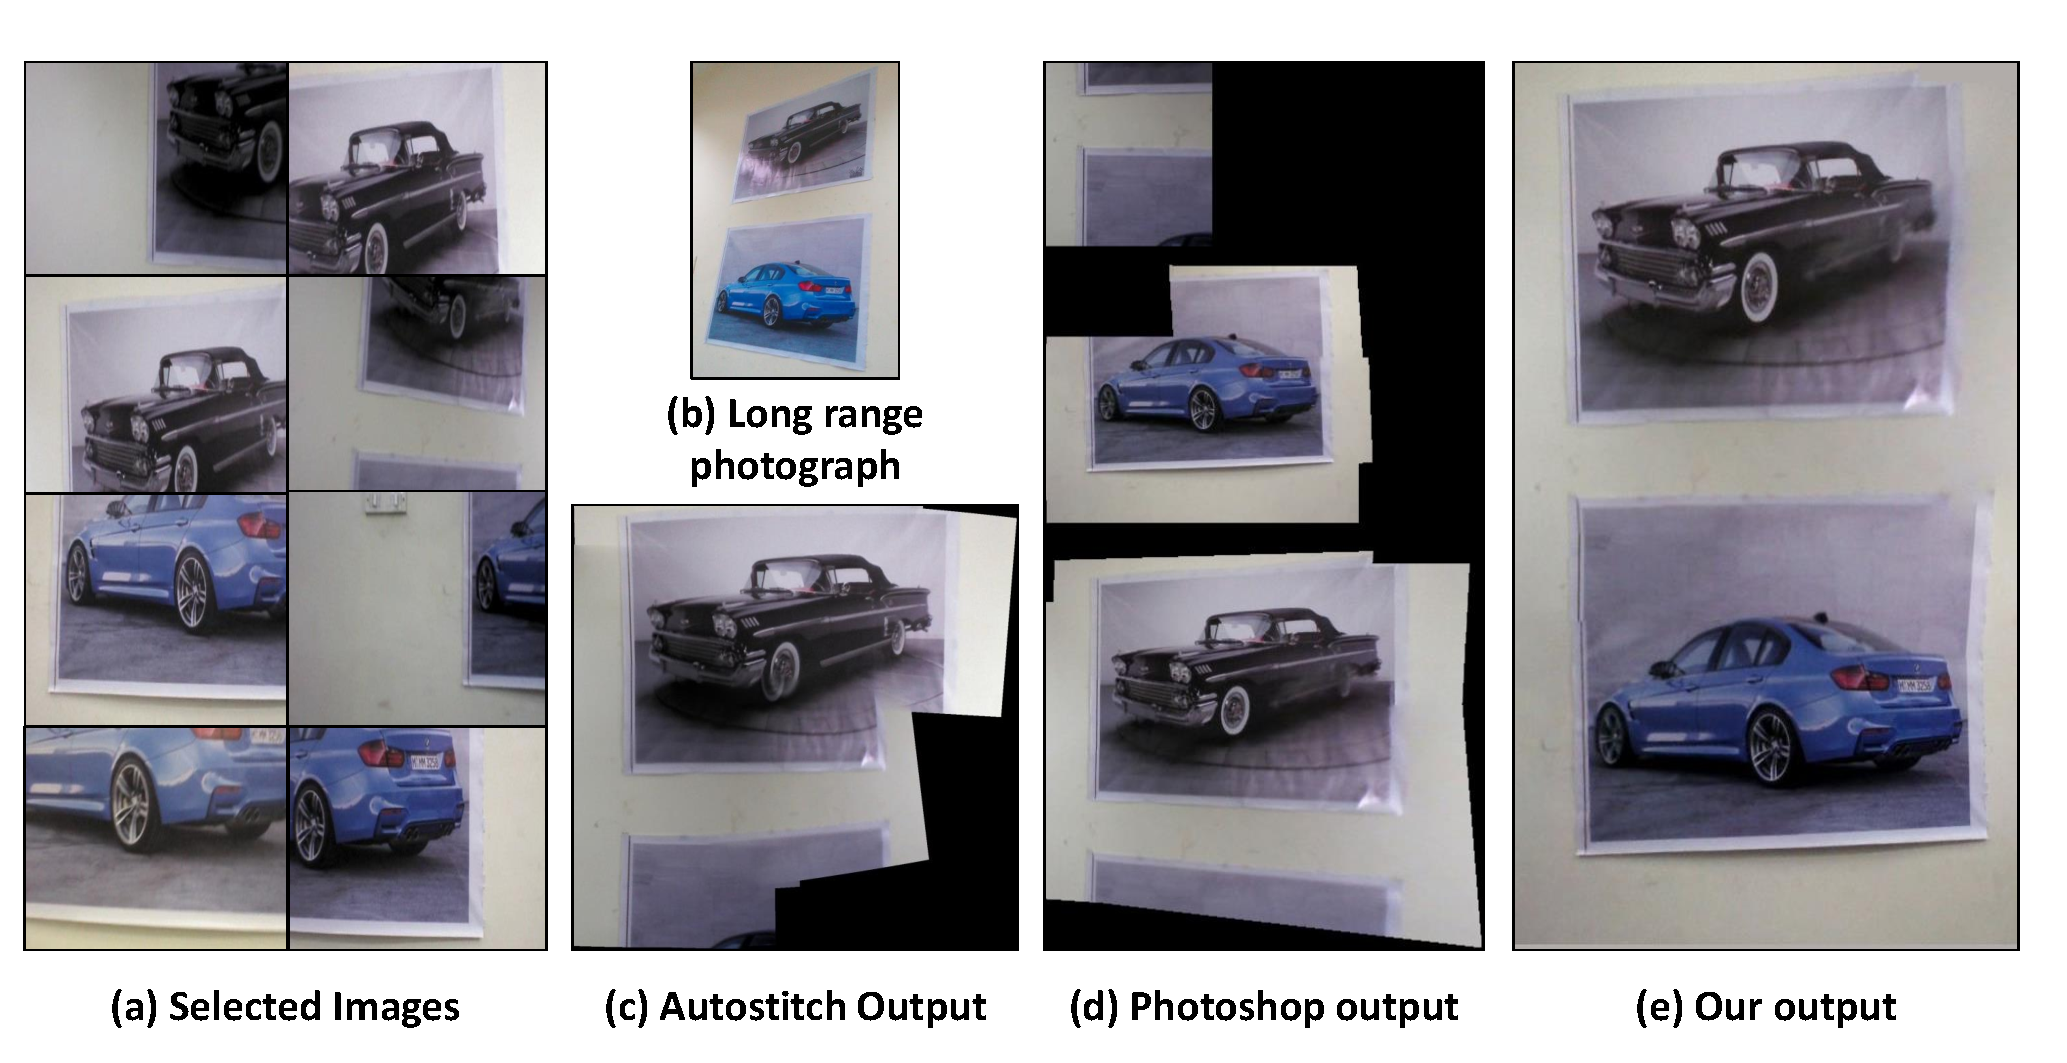
\includegraphics[width=0.98\linewidth]{figures/vacantSpaces/indoor_results}
	\caption[Result: Cars]{ (a) Pruned images from the quadcopter video using our
  saliency algorithm of (b) an indoor scene. This long-range photograph
  has been captured separately by a smartphone camera only for the
  context. Notice a significant vacant space in the imagery.  (c)
  The output of AutoStitch -- only the upper half of the scene is output.
  (d) The output of Adobe Photoshop CS6 -- the vacant space posed a problem to
  the feature matching algorithm, so instead of a mosaic, individual
  pieces were output as mini-panoramas (e) Our output on the selected
  images. We can present the scene in high fidelity in an orthographic view.}	
	\label{fig:vacantSpaces_result}
	\end{figure}
  
\subsection{Autonomous Multiplanar Imaging through Quadcopter}
\begin{figure}[h!]
\centering
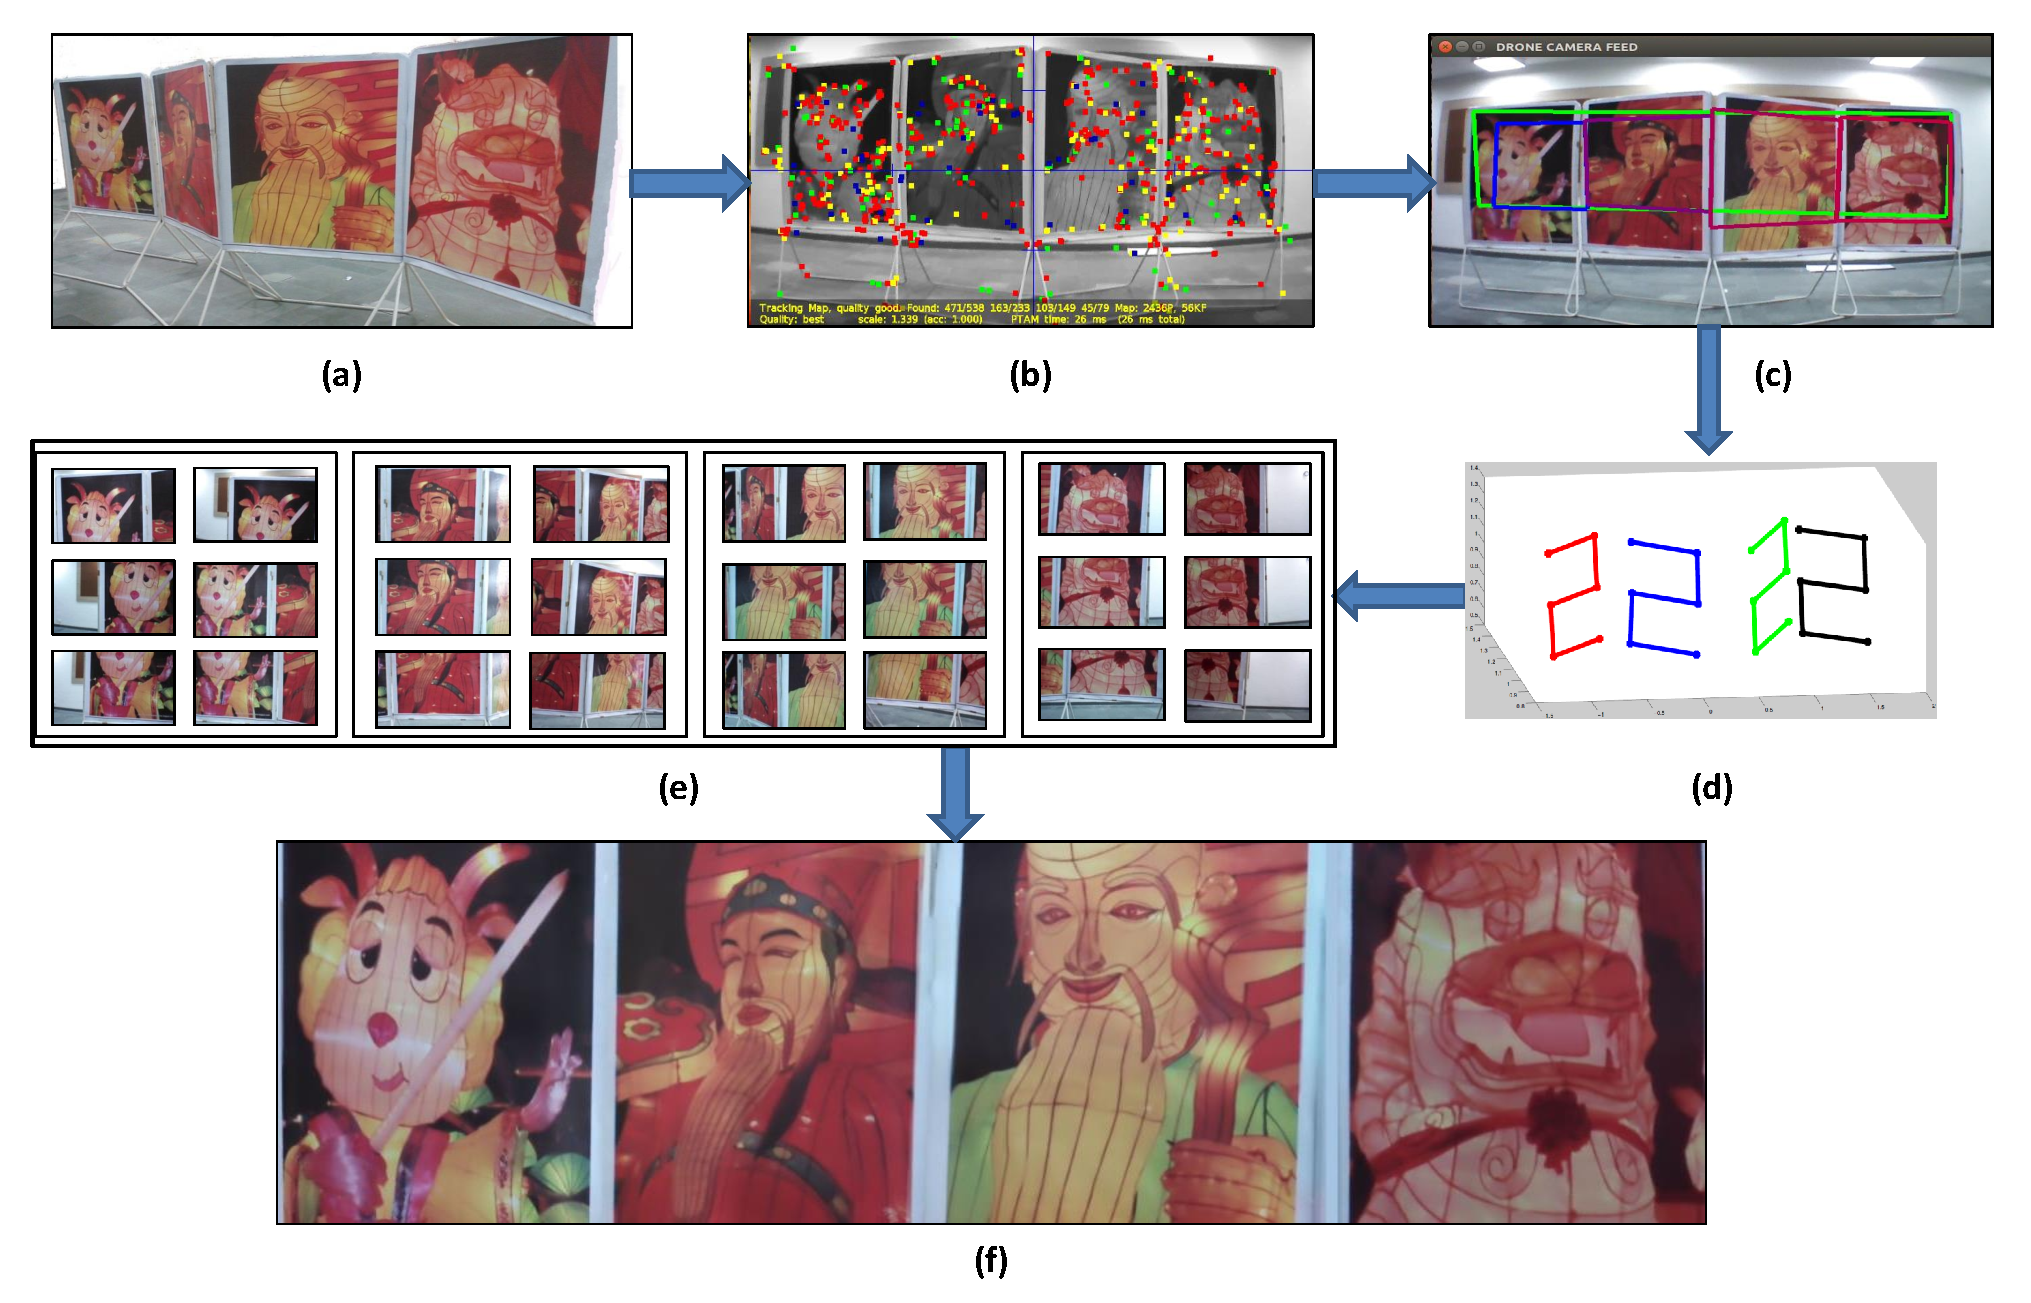
\includegraphics[width=0.98\linewidth]{figures/multiplanar/workflow}
\caption[Overflow of autonomous multiplanar imaging through quadcopter]{Overview
of multiplanar imaging through quadcopter:
(a) An input scene to be imaged.
(b) Feature points in the scene are found, and their 3D positions are estimated
using scale aware PTAM \cite{engel}. (c) Multiple planar bounded regions are
estimated using our algorithm. (d) For each bounded planar region, 3D camera
positions are calculated, and overall path planning is done. (e) Videos are
captured at each target position. From each captured video, the appropriate
frame is found. (f) Individual mosaics are joined to get the final output.}
\label{fig:multiplanar_workflow}
\end{figure}

Homography-based mosaicing algorithms can mosaic only if the scene lies on a single planar
surface. But the real world is made-up of multiplanar as well as curved surfaces.
In fact, we have many circumstances where the input scene is spread over
multiple planes. In such cases, we would like to image each planar region
orthographically and then `unroll' the whole scene by joining the individual
mosaics so that we get the output mosaic of the input scene as if it is present
on a single plane.

The method adopted is pictorially depicted in the overview shown in
Figure~\ref{fig:multiplanar_workflow}. In brief, we probe the input scene
through a quadcopter, calculate the 3D positions of feature points using PTAM
based method~\cite{engel}. Later, we use our algorithm, an improvement over
J-linkage~\cite{jlinkage} to detect multiplanar bounded regions from the area
marked by the user through our user interface. Path planning is done for each
planar bounded region to determine the camera positions in such a way that
images captured from those positions encompass the scene in an optimal manner.
The quadcopter is autonomously maneuvered along the estimated path and videos
are captured at target points. For each planar bounded region, the appropriate
frame from each video is found and then given to a mosaicing algorithm. 
Finally, all mosaics are joined to get a full unrolled view.

Our experiments are done on various setups covering multiple planes.
In one such experiment, paintings were arranged in the convex
fashion as shown in Figure~\ref{fig:multiplanar_result} (Top-Left). We have
selected the area to be imaged as shown in Figure \ref{fig:multiplanar_result}
(Top-Right). In the path planning stage, overall 30 (9 from the left plane, 12
from the middle plane, and 9 from the right plane) positions to cover full
region are estimated.  Images captured from those positions are mosaiced using our
algorithm to get the final mosaicing output as shown in the
Figure~\ref{fig:multiplanar_result} (Bottom).
\begin{figure}[h!]
	\centering
	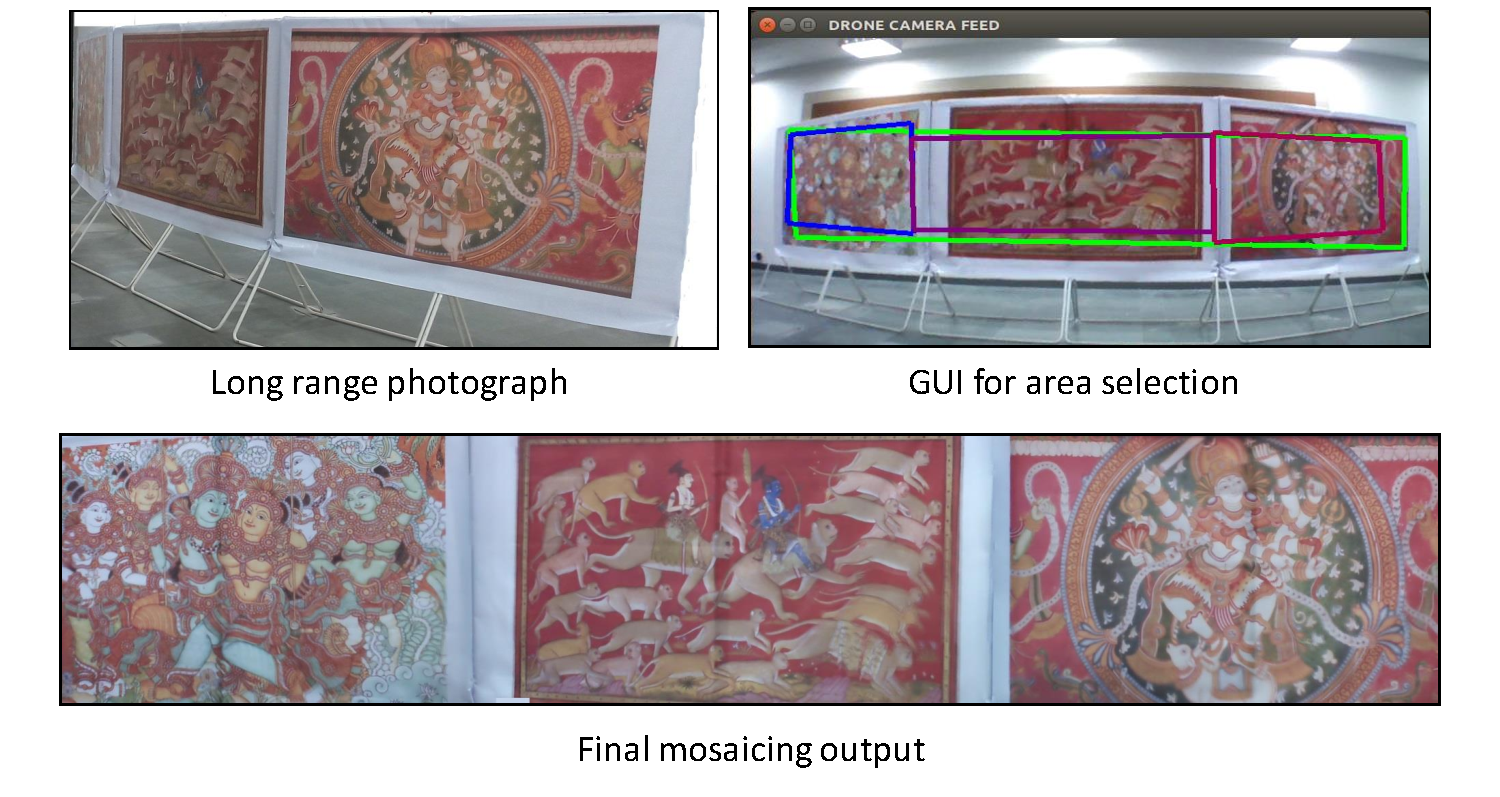
\includegraphics[width=0.98\linewidth]{figures/multiplanar/convexResult}
	\caption[Result: Imaging Convex Surface ]{The exhibition of 
	temple paintings arranged in convex fashion as shown in the long-range
	photograph (top-left). Note that we cannot cover all paintings with enough
	details simultaneously. We have selected the area to be imaged as shown in GUI
	for area selection (top-right). Green quadrilateral shows the user selected
	area while blue, violet and magenta colored quadrilaterals represent the
	multiple planar bounded regions estimated by our algorithm. In the path
	planning stage, overall 30 (9 from the left plane, 12 from the middle plane,
	and 9 from the right plane) positions are estimated to cover the full region.
	Images captured from the estimated positions are mosaiced using our algorithm to get
	the final mosaicing output as shown in the bottom image.}
	\label{fig:multiplanar_result}
\end{figure}
	
\subsection{Blur Resilient Fiducials for Quadcopter}

\begin{figure}[h!]
\centering
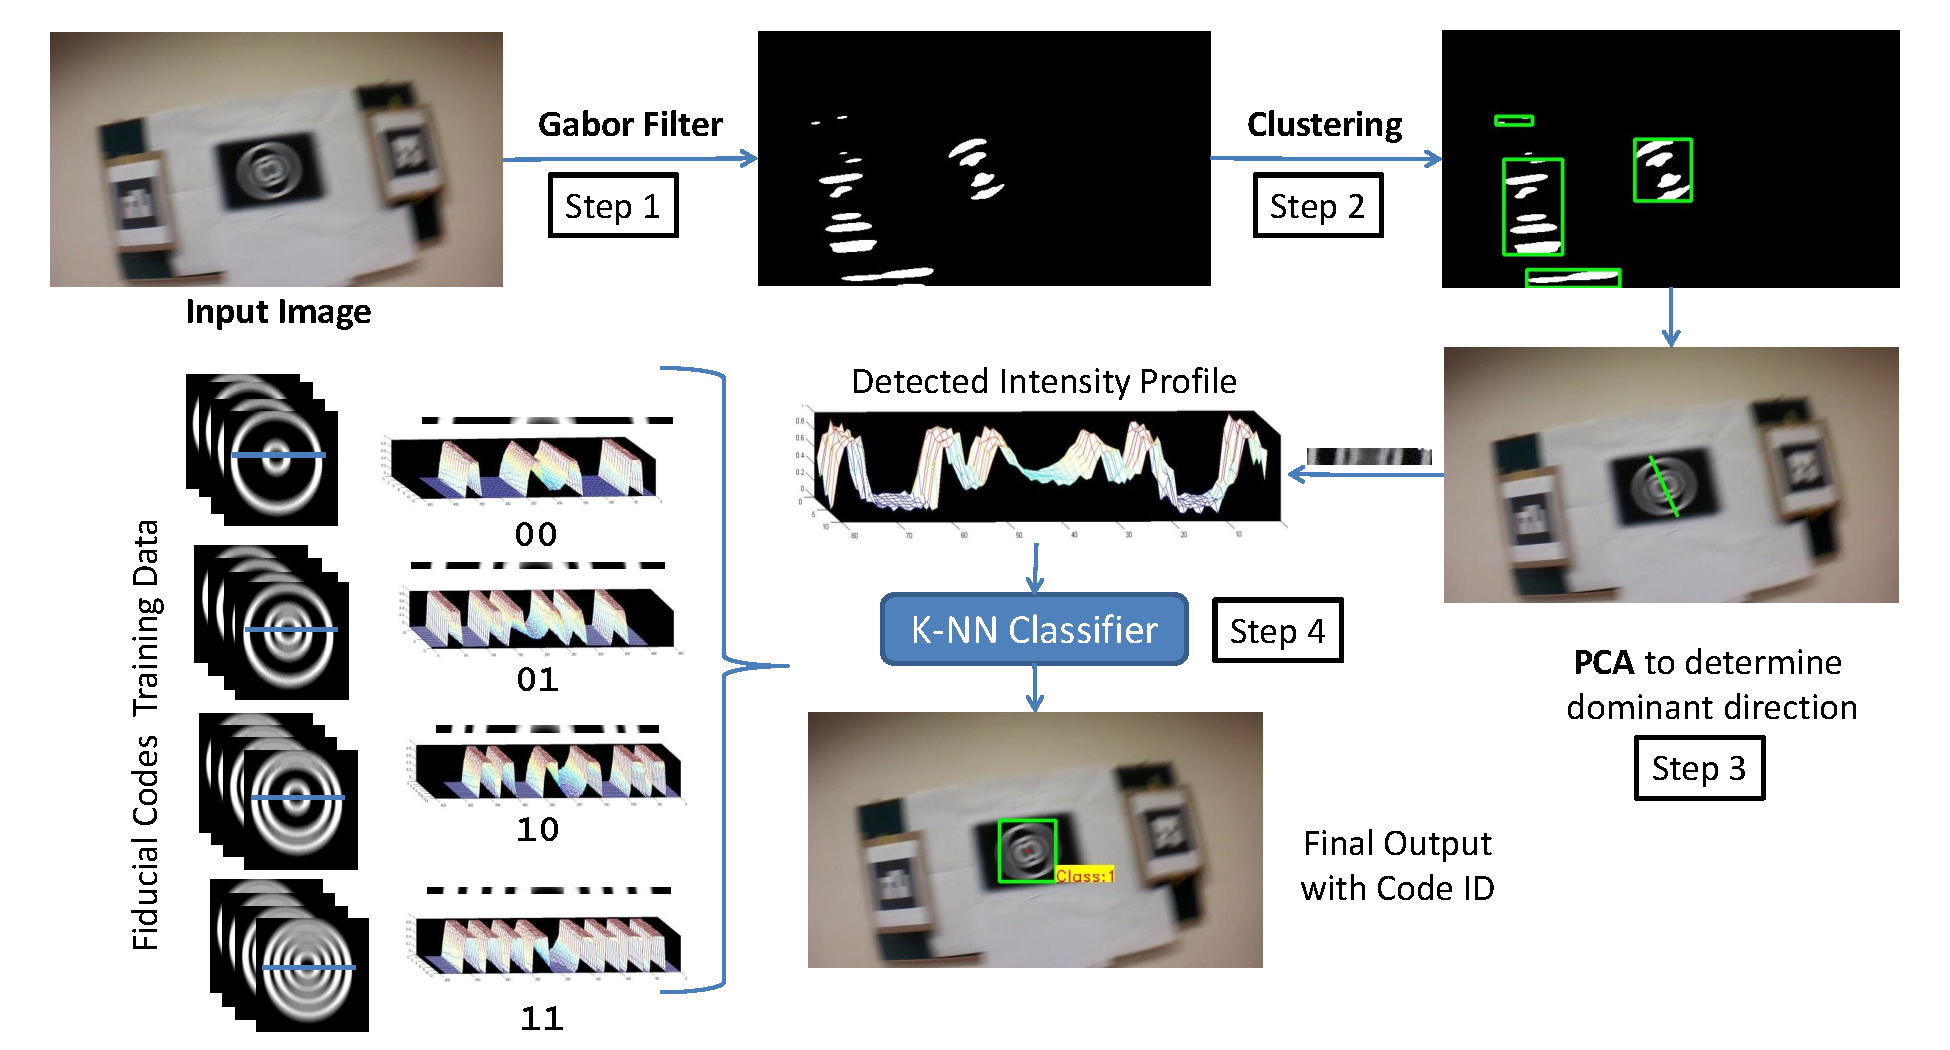
\includegraphics[width=0.98\linewidth]{figures/fiducial/overall_flow}
\caption[Overall Workflow of blur resilient fiducial recognition algorithm]{An
overview of our fiducial recognition algorithm.
    The four step process includes (Step 1) Filtering,
    (Step 2) Component clustering, (Step 3) Dominant direction determination,
    and (Step 4) Classification using prior training data.}
 \label{fig:fiducial_workflow}
\end{figure}

A single quadcopter is not sufficient for imaging large multiplanar scenes due
to energy constraints. Instead, we may use multiple quadcopters in
collaboration for imaging multiplanar scenes. In such cases, we have to identify
each quadcopter uniquely for accurate collaboration among multiple quadcopters. 

Generally, fiducial markers such as ARTag~\cite{Fiala05} are used to identify
objects in the environment.The low-cost quadcopters often exhibit very quick and 
erratic physical movements that result in motion blur which is evident in the images 
captured from the quadcopter's onboard camera. This motion blur has an adverse effect
on the recognition of fiducial markers. This can be seen in Figure~\ref{fig:fiducials_result} (Top) where the
ARTag fiducial cannot be recognized due to motion blur. This is not too
surprising as most existing fiducials are not designed to handle motion blur.

Compounding this problem is the additional issue of dropped video
frames from the quadcopter's wireless communication module. This means
that not only is blur a problem, but there may be large
discontinuities in the pattern's position due to missing video
frames. This latter problem makes it challenging to apply tracking algorithms
that can exploit temporal coherence for determining the fiducial's position.

To address these problems, we propose a fiducial that is designed to be
resilient to motion blur. Our design is based on circles as shown in
Figure~\ref{fig:fiducials_result} (Bottom). The design is based on the
observation that motion blur from a quadcopter tends to be linear in nature. As
such, when our fiducial is blurred, there is no blur in the direction
perpendicular to the direction of motion. This allows the signature of the
fiducial to remain intact in any direction.

Figure~\ref{fig:fiducial_workflow} shows the process involved in fiducial
recognition. Our recognition algorithm has four steps. In Step~1, we apply a Gabor
filter on the image to isolate the potential locations of the pattern.  In
Step~2, we find clusters of patches in the Gabor output.  In Step~3, we perform
the Principal Component Analysis (PCA) on each cluster to find the dominant
direction unaffected by the blur.  Finally in Step~4, based on the direction
detected, we extract the intensity profile of the pattern and classify the
fiducial.

\begin{figure}
\begin{subfigure}[b]{0.24\textwidth}
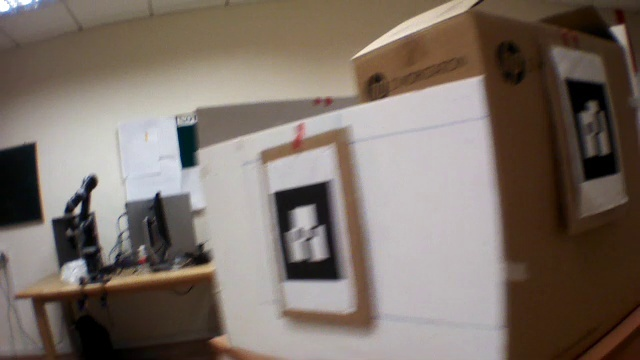
\includegraphics[width=\linewidth]{figures/fiducial/setup_artag/output_79.jpg}
\end{subfigure}
\begin{subfigure}[b]{0.24\textwidth}
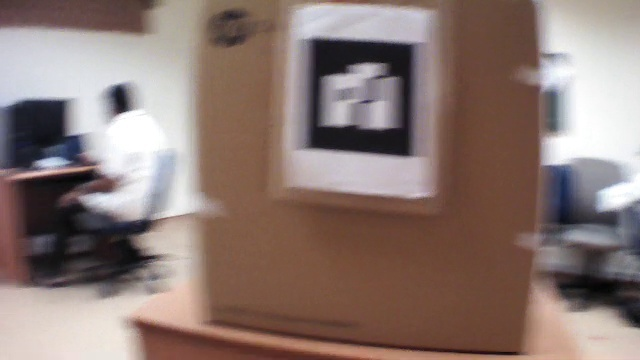
\includegraphics[width=\linewidth]{figures/fiducial/setup_artag/output_150.jpg}
\end{subfigure}
\begin{subfigure}[b]{0.24\textwidth}
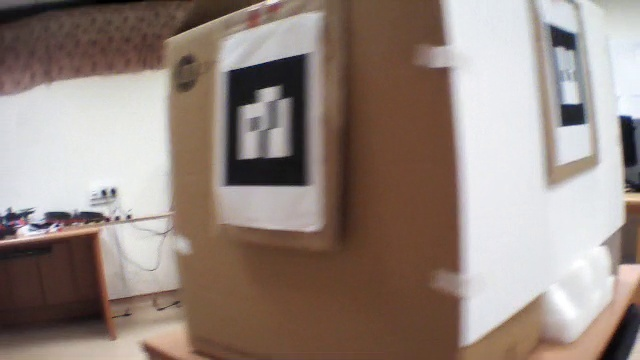
\includegraphics[width=\linewidth]{figures/fiducial/setup_artag/output_194.jpg}
\end{subfigure}
\begin{subfigure}[b]{0.24\textwidth}
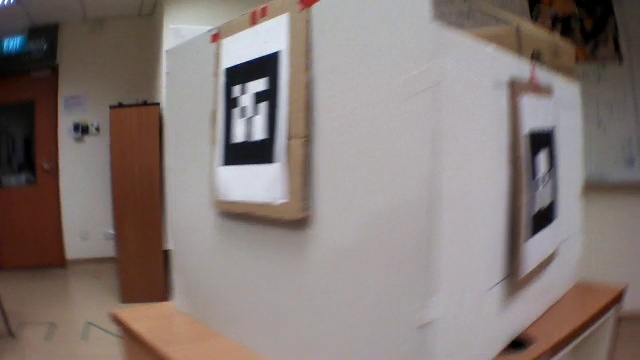
\includegraphics[width=\linewidth]{figures/fiducial/setup_artag/output_480.jpg}
\end{subfigure}\\
\begin{subfigure}[b]{0.24\textwidth}
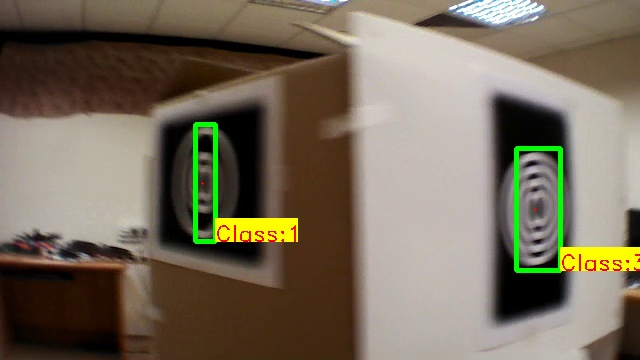
\includegraphics[width=\linewidth]{figures/fiducial/setup_our/output_6/output_514.jpg}
\end{subfigure}
\begin{subfigure}[b]{0.24\textwidth}
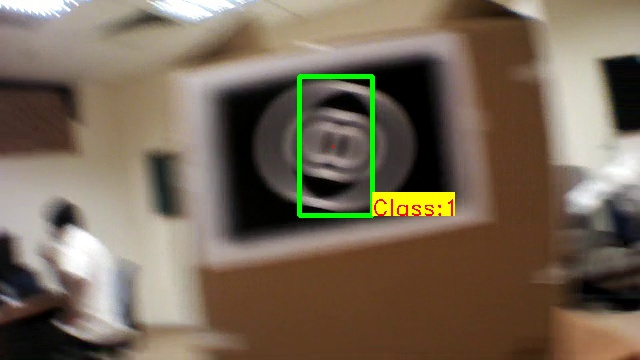
\includegraphics[width=\linewidth]{figures/fiducial/setup_our/output_2/output_64.jpg}
\end{subfigure}
\begin{subfigure}[b]{0.24\textwidth}
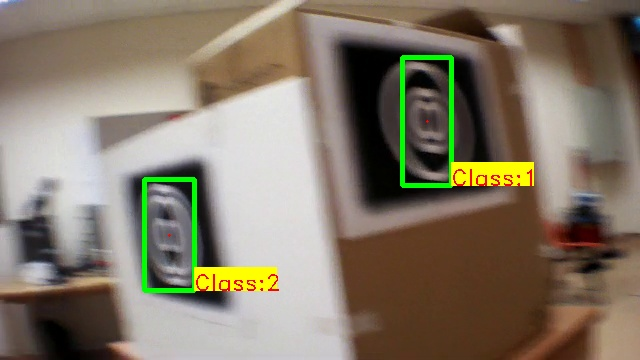
\includegraphics[width=\linewidth]{figures/fiducial/setup_our/output_2/output_35.jpg}
\end{subfigure}
\begin{subfigure}[b]{0.24\textwidth}
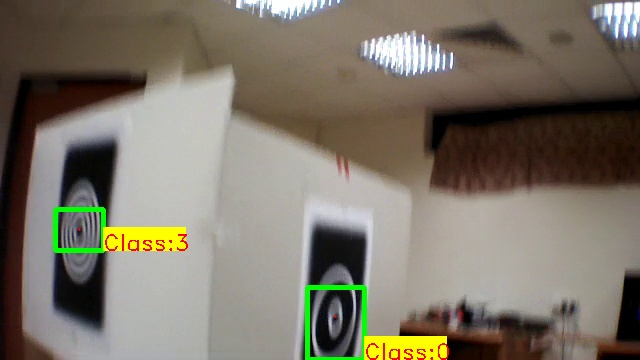
\includegraphics[width=\linewidth]{figures/fiducial/setup_our/output_6/output_943.jpg}
\end{subfigure}
\caption[Comparison of ARTag and our fiducial when quadcopter is
  revolving around our setup]{Comparison of ARTag and our fiducial when quadcopter is
  revolving around our setup. 
\textbf{Top} ARTags are not recognized, shown by an absence of green rectangles.
\textbf{Bottom} In similar conditions, proposed fiducials are successfully
recognized. The overall recognition rate of proposed fiducials is 90\% while that
of ARTags is around 60\%. }
\label{fig:fiducials_result}
\end{figure}
	
\section{Organization of the thesis}
The remainder of the thesis is organized as follows:\\

\noindent \textbf{Chapter 2} explains the details of a quadcopter focussing on
control and navigation aspects. Here, we also present previously published work
in the area of mosaicing, autonomous navigation of quadcopter as well as
fiducials. We use this chapter as an opportunity to establish and contrast the
scope of this thesis with respect to prior art.\\

\noindent \textbf{Chapter 3} elaborates our proposed method for mosaicing
scenes with vacant spaces using quadcopter. Proposed method fuses positional
information from quadcopter with images to first, find out the position from which each
image is taken and accordingly sort the images in two dimensional grid; second,
use positional information to join two adjacent images which have very few features
in common (and hence cannot be stitched using the homography-based method).\\

\noindent \textbf{Chapter 4} provides an overview of our approach
for imaging multiplanar scenes through quadcopter. Issues such as detection of
multiplanar bounded regions and path planning for efficient imaging of multiplanar scenes
are addressed.\\

\noindent \textbf{Chapter 5} elaborates on our design of blur
resilient fiducial for identification of objects under a heavy motion blur. We
have also proposed algorithm for robust recognition of our blur resilient
fiducial in this chapter.\\
 
 \noindent \textbf{Chapter 6} concludes the thesis by summarizing our
 contributions.
  We have also discussed possible ways to extend some of the ideas proposed in this thesis.
